%%%%%%%%%%%%%%%%%%%%%%%%%%%%%%%%%%%%%%%%%
% Beamer Presentation
% LaTeX Template
% Version 1.0 (10/11/12)
%
% This template has been downloaded from:
% http://www.LaTeXTemplates.com
%
% License:
% CC BY-NC-SA 3.0 (http://creativecommons.org/licenses/by-nc-sa/3.0/)
%
%%%%%%%%%%%%%%%%%%%%%%%%%%%%%%%%%%%%%%%%%

%----------------------------------------------------------------------------------------
%	PACKAGES AND THEMES
%----------------------------------------------------------------------------------------

\documentclass{beamer}

\mode<presentation> {

% The Beamer class comes with a number of default slide themes
% which change the colors and layouts of slides. Below this is a list
% of all the themes, uncomment each in turn to see what they look like.

%\usetheme{default}
%\usetheme{AnnArbor}
%\usetheme{Antibes}
%\usetheme{Bergen}
%\usetheme{Berkeley}
%\usetheme{Berlin}
\usetheme{Boadilla}
%\usetheme{CambridgeUS}
%\usetheme{Copenhagen}
%\usetheme{Darmstadt}
%\usetheme{Dresden}
%\usetheme{Frankfurt}
%\usetheme{Goettingen}
%\usetheme{Hannover}
%\usetheme{Ilmenau}
%\usetheme{JuanLesPins}
%\usetheme{Luebeck}
%\usetheme{Madrid}
%\usetheme{Malmoe}
%\usetheme{Marburg}
%\usetheme{Montpellier}
%\usetheme{PaloAlto}
%\usetheme{Pittsburgh}
%\usetheme{Rochester}
%\usetheme{Singapore}
%\usetheme{Szeged}
%\usetheme{Warsaw}

% As well as themes, the Beamer class has a number of color themes
% for any slide theme. Uncomment each of these in turn to see how it
% changes the colors of your current slide theme.

\setbeamercolor{normal text}{fg=white, bg=black}


%\usecolortheme{albatross}
\usecolortheme{beaver}
%\usecolortheme{beetle}
%\usecolortheme{crane}
%\usecolortheme{dolphin}
%\usecolortheme{dove}
%\usecolortheme{fly}
%\usecolortheme{lily}
%\usecolortheme{orchid}
%\usecolortheme{rose}
%\usecolortheme{seagull}
%\usecolortheme{seahorse}
%\usecolortheme{whale}
%\usecolortheme{wolverine}

\setbeamercolor{title}{bg=black}
\setbeamercolor{title in head/foot}{bg=black!30}
%\setbeamercolor{author}{fg=black}
\setbeamercolor{frametitle}{bg=black}
%\setbeamercolor{author in head/foot}{bg=black}
%\setbeamercolor{institute in head/foot}{fg=item.fg!35}
\setbeamercolor{date in head/foot}{bg=black!45}
%\setbeamercolor{navigation symbols}{fg=gray}
%\setbeamercolor{item projected}{fg=black}
%\setbeamertemplate{blocks}[rounded][shadow=false]
%\setbeamertemplate{enumerate items}[circle]
\setbeamercolor{normal text}{fg=white,bg=black!97}
%\setbeamercolor{structure}{fg=white}
%\setbeamercolor{alerted text}{fg=red!85!black}
%\setbeamercolor{item projected}{use=item,fg=black,bg=item.fg!35}
%\setbeamercolor*{palette primary}{use=structure,fg=structure.fg}
%\setbeamercolor*{palette secondary}{use=structure,fg=structure.fg!95!black}
%\setbeamercolor*{palette tertiary}{use=structure,fg=structure.fg!90!black}
%\setbeamercolor*{palette quaternary}{use=structure,fg=structure.fg!95!black,bg=black!80}
%\setbeamercolor*{framesubtitle}{fg=white}
%\setbeamercolor*{block title}{parent=structure,bg=black!60}
%\setbeamercolor*{block body}{fg=black,bg=black!10}
%\setbeamercolor*{block title alerted}{parent=alerted text,bg=black!15}
%\setbeamercolor*{block title example}{parent=example text,bg=black!15}

%\setbeamertemplate{footline} % To remove the footer line in all slides uncomment this line
%\setbeamertemplate{footline}[page number] % To replace the footer line in all slides with a simple slide count uncomment this line

%\setbeamertemplate{navigation symbols}{} % To remove the navigation symbols from the bottom of all slides uncomment this line
}

\usepackage{graphicx} % Allows including images
\usepackage{booktabs} % Allows the use of \toprule, \midrule and \bottomrule in tables

%adding video package
\usepackage{media9}
\usepackage[utf8]{inputenc}
\usepackage[T1]{fontenc}
\usepackage{parskip}
%\usepackage{multimedia}
\usepackage{pdfpc-commands}
%----------------------------------------------------------------------------------------
%	TITLE PAGE
%----------------------------------------------------------------------------------------

\title[Detonation Initiation]{Turbulently-Driven Detonation Initiation in Electron-Degenerate Matter with Helium} % The short title appears at the bottom of every slide, the full title is only on the title page

\author{Gabriel Casabona} % Your name
\institute[UMassD] % Your institution as it will appear on the bottom of every slide, may be shorthand to save space
{
University of Massachusetts Dartmouth \\ % Your institution for the title page
\medskip
\textit{MS Thesis Defense} \\ % Your email address
\medskip
Thesis Adviser: Robert Fisher, Ph.D.
}
\date{\today} % Date, can be changed to a custom date

\begin{document}

\begin{frame}
\titlepage % Print the title page as the first slide
\end{frame}

%\begin{frame}
%\frametitle{Overview} % Table of contents slide, comment this block out to remove it
%\tableofcontents % Throughout your presentation, if you choose to use \section{} and \subsection{} commands, these will automatically be printed on this slide as an overview of your presentation
%\end{frame}

%----------------------------------------------------------------------------------------
%	PRESENTATION SLIDES
%----------------------------------------------------------------------------------------

%------------------------------------------------
\section{First Section} % Sections can be created in order to organize your presentation into discrete blocks, all sections and subsections are automatically printed in the table of contents as an overview of the talk
%------------------------------------------------

\subsection{Subsection Example} % A subsection can be created just before a set of slides with a common theme to further break down your presentation into chunks

%\begin{frame}
%\frametitle{Paragraphs of Text}
%Sed iaculis dapibus gravida. Morbi sed tortor erat, nec interdum arcu. Sed id lorem lectus. Quisque viverra augue id sem ornare non aliquam nibh tristique. Aenean in ligula nisl. Nulla sed tellus ipsum. Donec vestibulum ligula non lorem vulputate fermentum accumsan neque mollis.\\~\\

%Sed diam enim, sagittis nec condimentum sit amet, ullamcorper sit amet libero. Aliquam vel dui orci, a porta odio. Nullam id suscipit ipsum. Aenean lobortis commodo sem, ut commodo leo gravida vitae. Pellentesque vehicula ante iaculis arcu pretium rutrum eget sit amet purus. Integer ornare nulla quis neque ultrices lobortis. Vestibulum ultrices tincidunt libero, quis commodo erat ullamcorper id.
%\end{frame}

%------------------------------------------------

\begin{frame}
	\frametitle{Outline}
	\begin{itemize}
		\item What is a Type Ia Supernova (SNe Ia)?
		\item Stellar Lifetime
		\item White Dwarf
		\item Deflagration to Detonation Transition
		\item Zel'dovich Gradient Mechanism
		\item Carbon Detonation
		\item Helium Detonation
		\item Nuclear Physics
		\item Method
		\item Results
	\end{itemize}
\end{frame}



%------------------------------------------------


\begin{frame}
\frametitle{Type Ia Supernova}

\begin{columns}[c]
        \column{0.5\textwidth}
	\begin{itemize}
		\item Strong silicon lines in the absence of hydrogen
		\item Used as standardizable candles
		\item Led to the discovery of the accelerated expansion of the universe
		\item Cosmic Rays
	\end{itemize}


\column{0.5\textwidth}
        \begin{figure}
    \begin{center}
      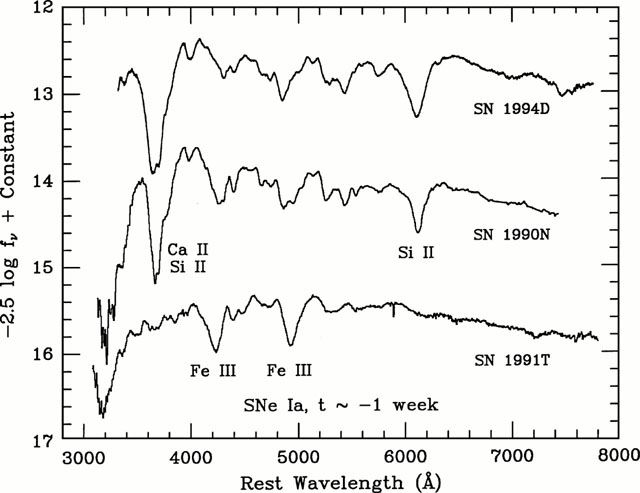
\includegraphics[width=.90\linewidth]{spectrum.jpg}
	    \caption{Fillipenko}
    \end{center}
  \end{figure}

        \end{columns}

\end{frame}

%------------------------------------------------

\begin{frame}
\frametitle{Type Ia Supernova}

\begin{columns}[c]
        \column{0.5\textwidth}
        \begin{itemize}
                \item SN 2011fe confirmed that a compact object must be the progenitor of a SNe Ia
        \end{itemize}


\column{0.5\textwidth}
        \begin{figure}
    \begin{center}
      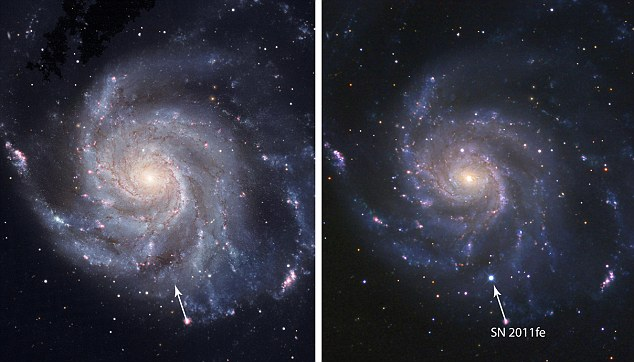
\includegraphics[width=.90\linewidth]{2011fe.jpg}
            \caption{2011fe as seen by the Palomar Transient Factory}
    \end{center}
  \end{figure}

        \end{columns}

\end{frame}


%------------------------------------------------

\begin{frame}
\frametitle{Type Ia Supernova}

        \begin{figure}
    \begin{center}
      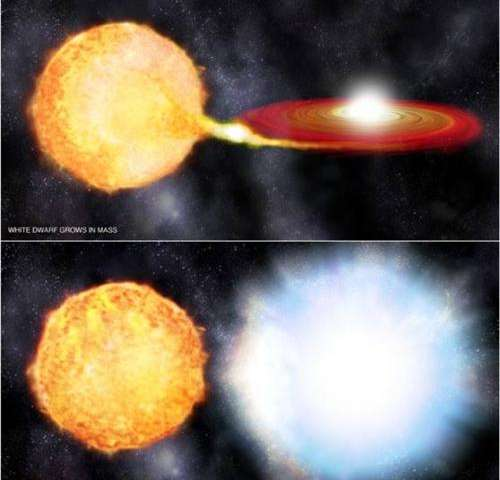
\includegraphics[width=.60\linewidth]{binary.jpg}
    \end{center}
		\begin{center}
			NASA/CXC/M Weiss
		\end{center}
  \end{figure}


\end{frame}



%------------------------------------------------

\begin{frame}
\frametitle{Stellar Lifetime}

        \begin{figure}
    \begin{center}
      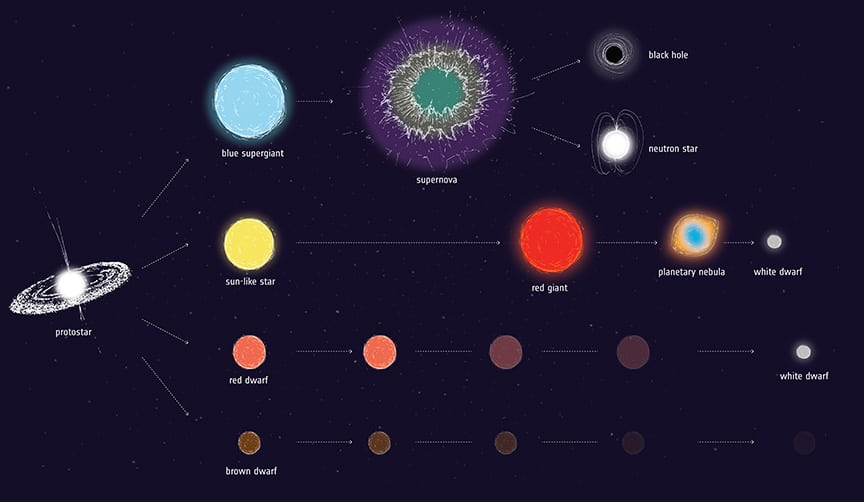
\includegraphics[width=.90\linewidth]{SE.jpg}
    \end{center}
  \end{figure}


\end{frame}


%------------------------------------------------

\begin{frame}
\frametitle{White Dwarf}

\begin{columns}[c]
        \column{0.5\textwidth}
        \begin{itemize}
                \item Degeneracy Pressure
		\item Causes volume to decrease as mass increases
		\item Chandrasekhar Mass Limit \\ $\simeq$ 1.4 $M_{solar}$
        \end{itemize}


\column{0.5\textwidth}
        \begin{figure}
    \begin{center}
      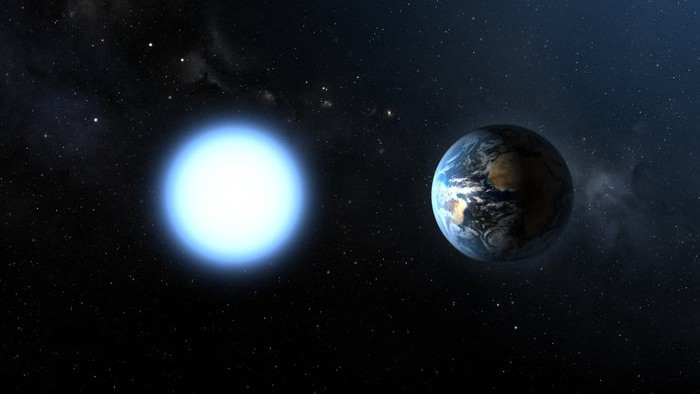
\includegraphics[width=.90\linewidth]{white_dwarf.jpeg}
	    \caption{Sirius B compared to Earth (European Space Agency)}
    \end{center}
  \end{figure}

        \end{columns}

\end{frame}



%------------------------------------------------

\begin{frame}
\frametitle{Deflagration to Detonation Transition}

\begin{columns}[c]
        \column{0.5\textwidth}
\begin{figure}
    \begin{center}
      \includegraphics[width=.70\linewidth]{fire.jpeg}
    \end{center}
  \end{figure}


\column{0.5\textwidth}
        \begin{figure}
    \begin{center}
      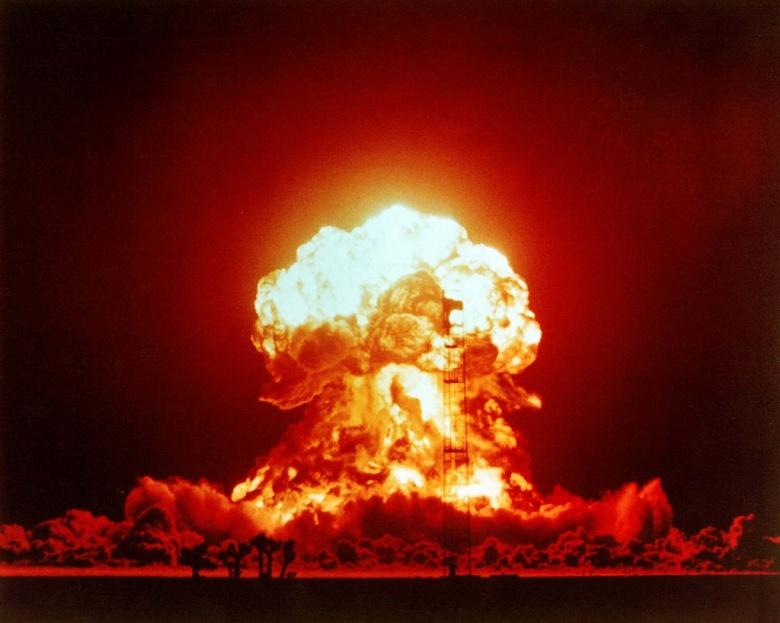
\includegraphics[width=.90\linewidth]{nuke.jpg}
    \end{center}
  \end{figure}

        \end{columns}

\end{frame}

%------------------------------------------------

\begin{frame}
\frametitle{Zel'dovich Gradient Mechanism}
        \vspace{20pt}

        \begin{center}
                \inlineMovie[loop]{ZGM_fail_slow.mp4}{ZGM_fail_slow.png}{height=0.6\textheight}
        \end{center}
        \begin{center}
                Failed detonation
        \end{center}
\end{frame}

%------------------------------------------------

\begin{frame}
        \frametitle{Zel'dovich Gradient Mechanism}

        \vspace{20pt}
        \begin{center}
                \inlineMovie[loop]{ZGM_success_slow.mp4}{ZGM_success_slow.png}{height=0.6\textheight}

        \caption{Successful Detonation}
        \end{center}

\end{frame}






%------------------------------------------------

\begin{frame}
\frametitle{Turbulence}

        \begin{figure}
    \begin{center}
      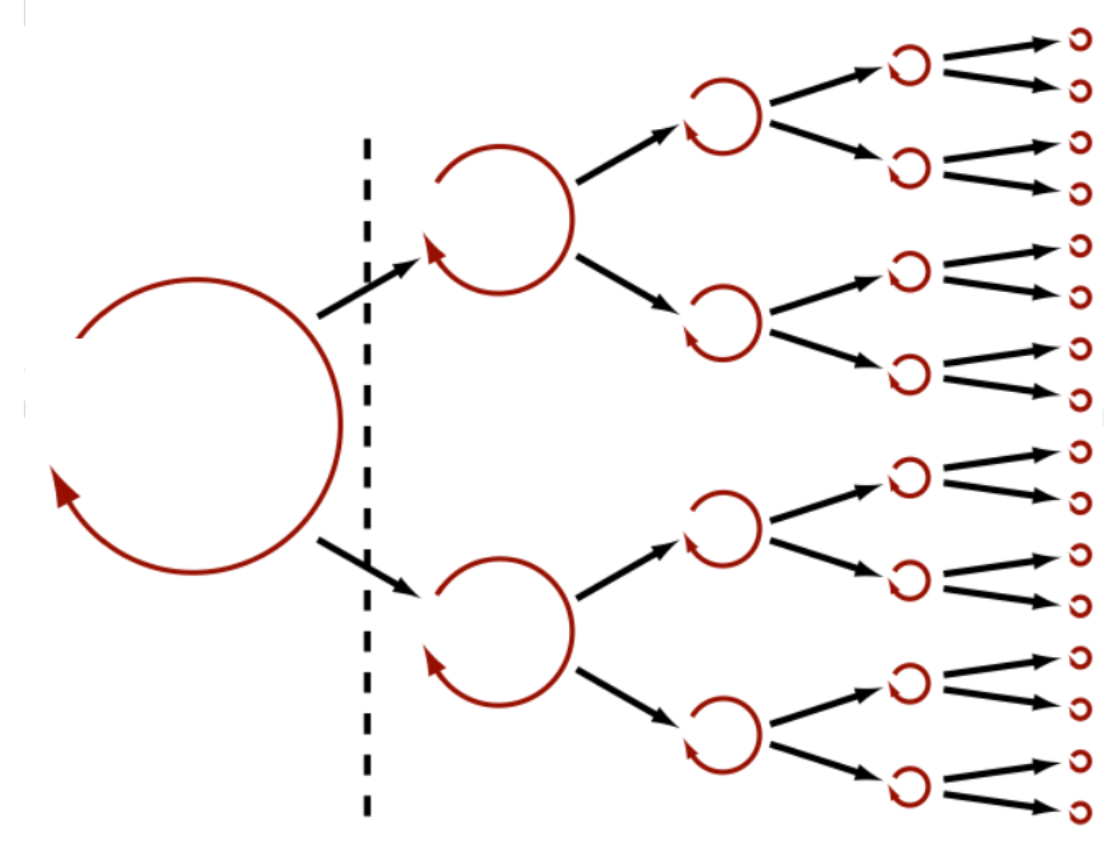
\includegraphics[width=.70\linewidth]{k41.png}
    \end{center}
		\begin{center}
			Kolmogorov's Theory (1941)
		\end{center}
  \end{figure}


\end{frame}

%------------------------------------------------

\begin{frame}
\frametitle{Carbon Detonation}

\begin{columns}[c]
        \column{0.5\textwidth}
        \begin{itemize}
		\item Highly Turbulent (Re $\simeq 10^{15}$) 
                \item Karlovitz Number
			\begin{itemize}
				\item Ka = (nuclear time scale/smallest turbulent time scale) $\simeq$ 8000
				\item \underline{Distributed Burning Regime}
			\end{itemize}
		\item Turbulent dissipation of energy dominates nuclear burning prior to detonation by up to 20 orders of magnitude
        \end{itemize}


\column{0.5\textwidth}
	\vspace{25pt}
        \begin{figure}
    \begin{center}
      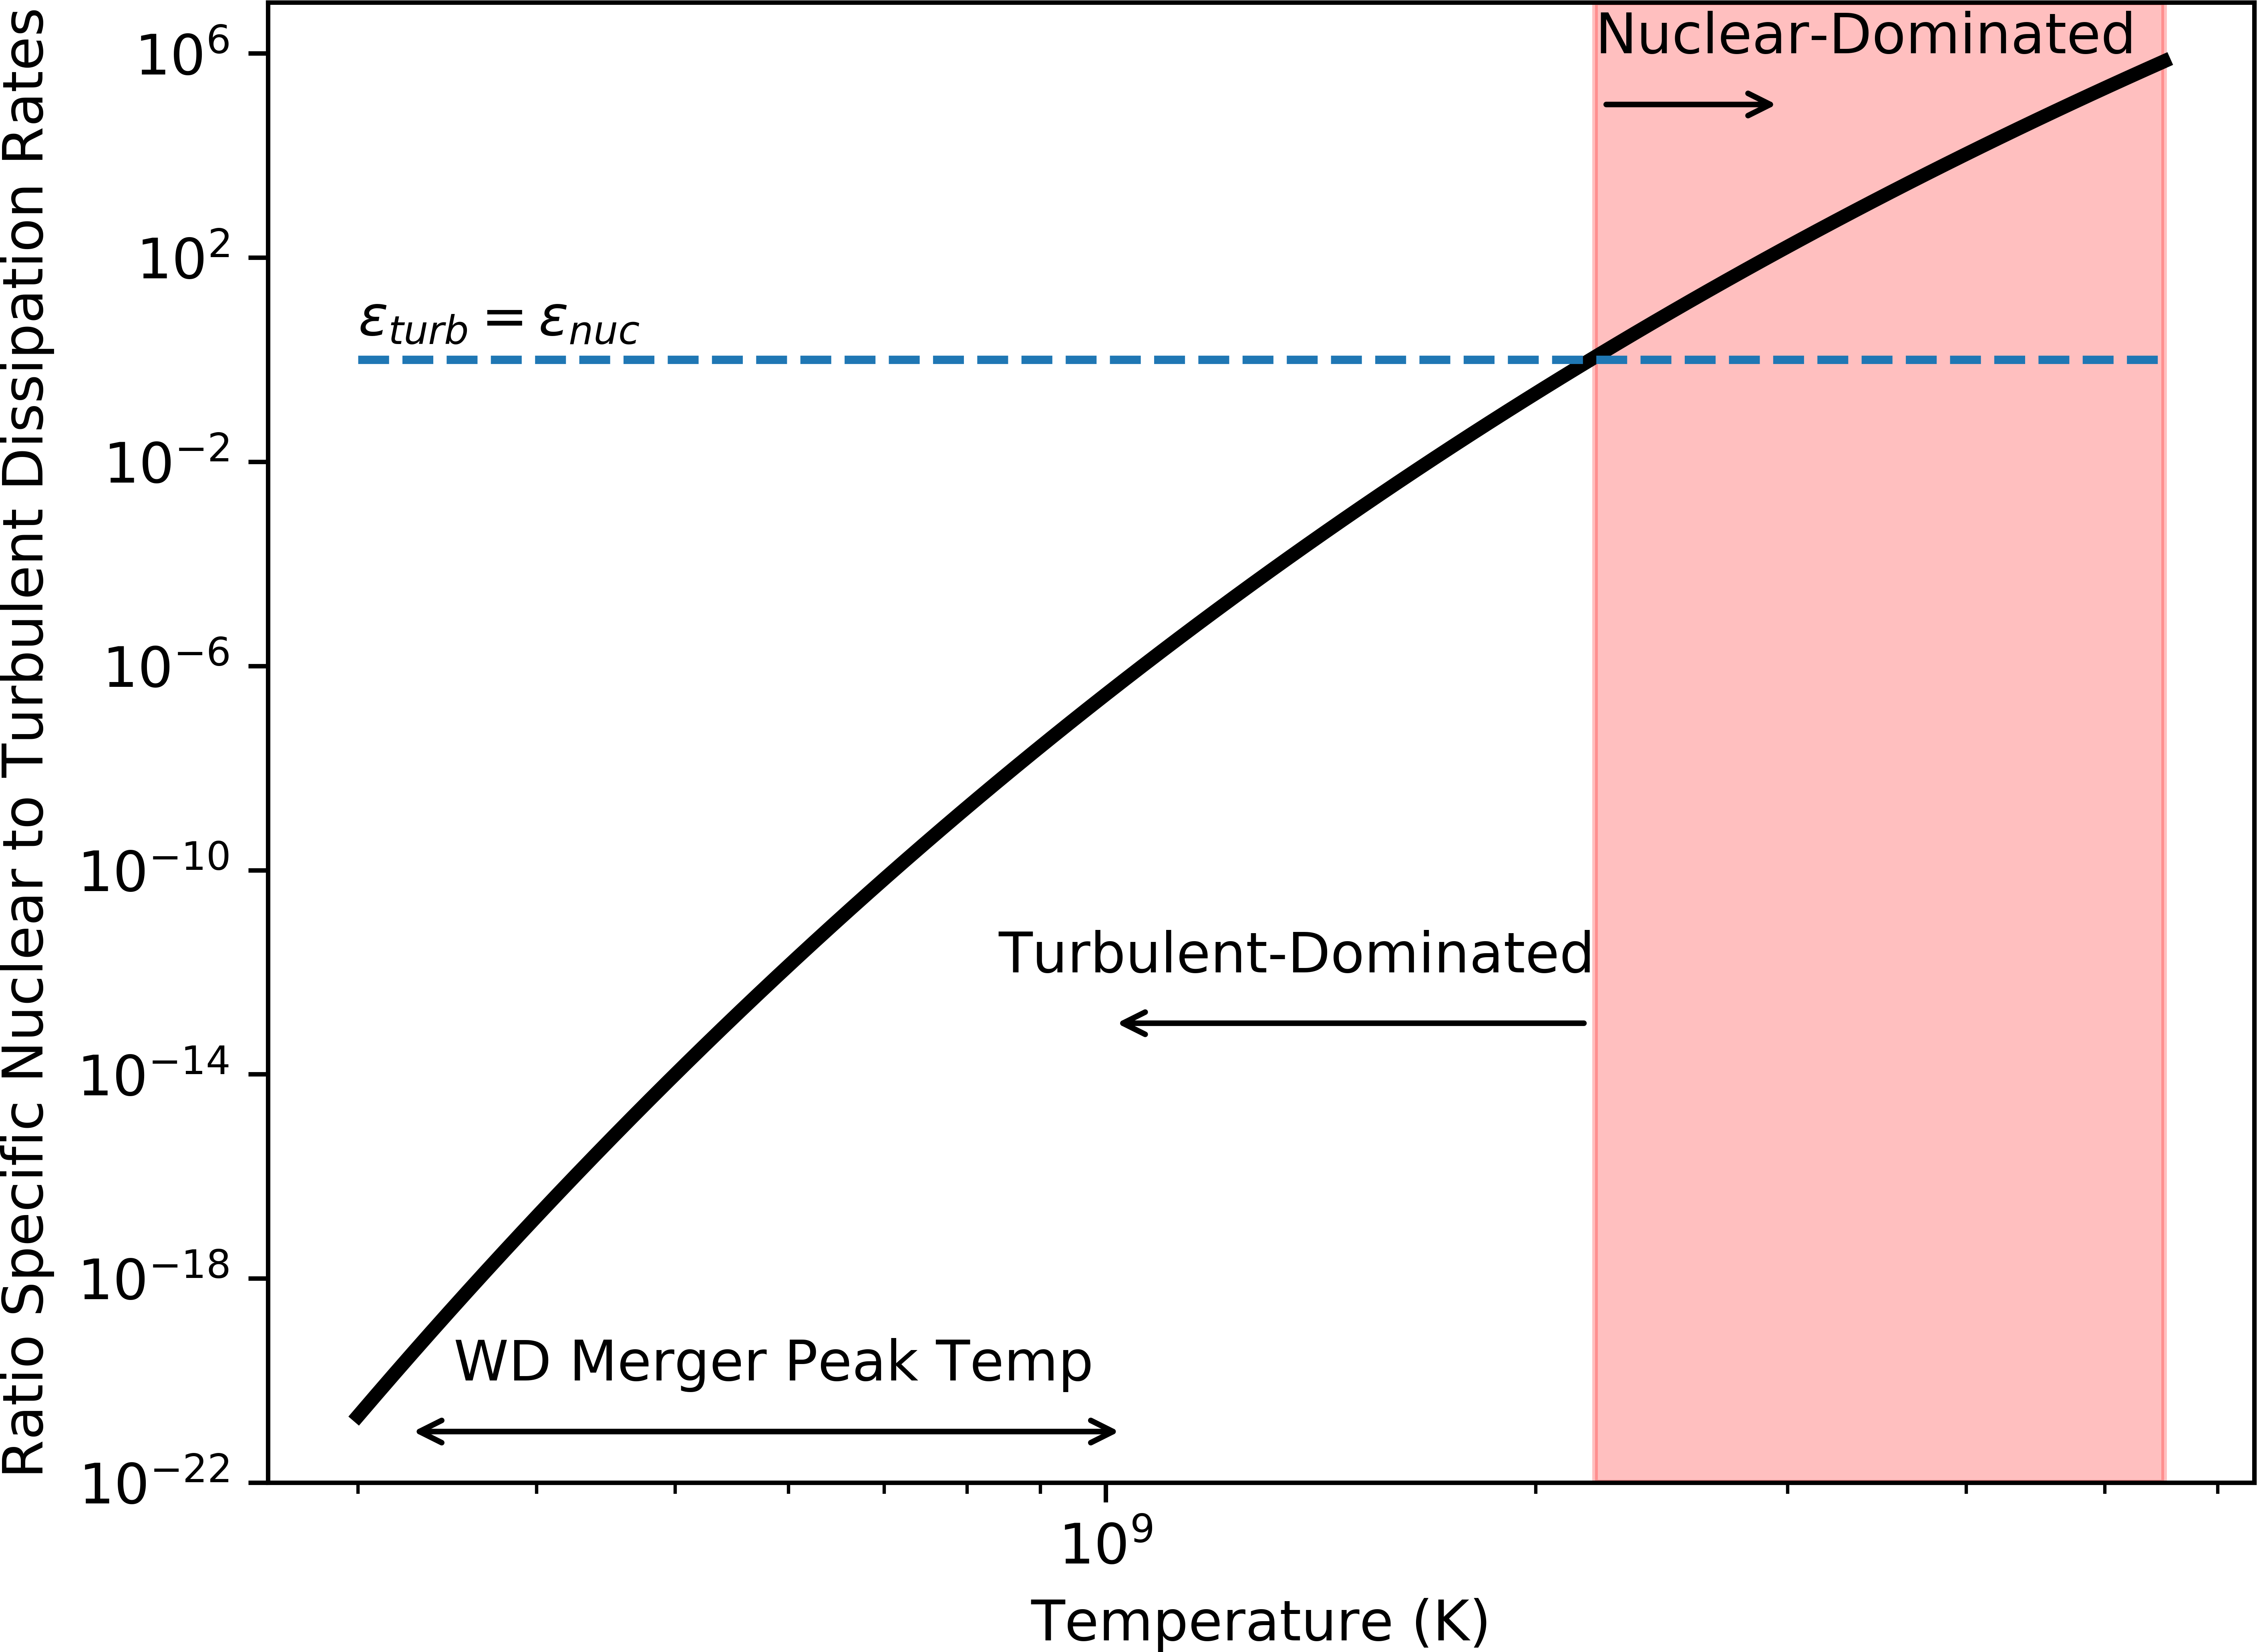
\includegraphics[width=.90\linewidth]{carbon_enuc_ration.png}
            \caption{Analytic Curve for Carbon Detonation}
    \end{center}
  \end{figure}

        \end{columns}

\end{frame}



%------------------------------------------------

\begin{frame}
\frametitle{Carbon Detonation}

\begin{columns}[c]
        \column{0.5\textwidth}
        \begin{itemize}
                \item Turbulently-Driven Detonation Mechanism of Carbon
                \item Fisher RT, Mozumdar P, Casabona G. 2019. Carbon Detonation Initiation in Turbulent Electron-Degenerate Matter. The Astrophysical Journal.
        \end{itemize}


\column{0.5\textwidth}
	\vspace{25pt}
        \begin{figure}
    \begin{center}
      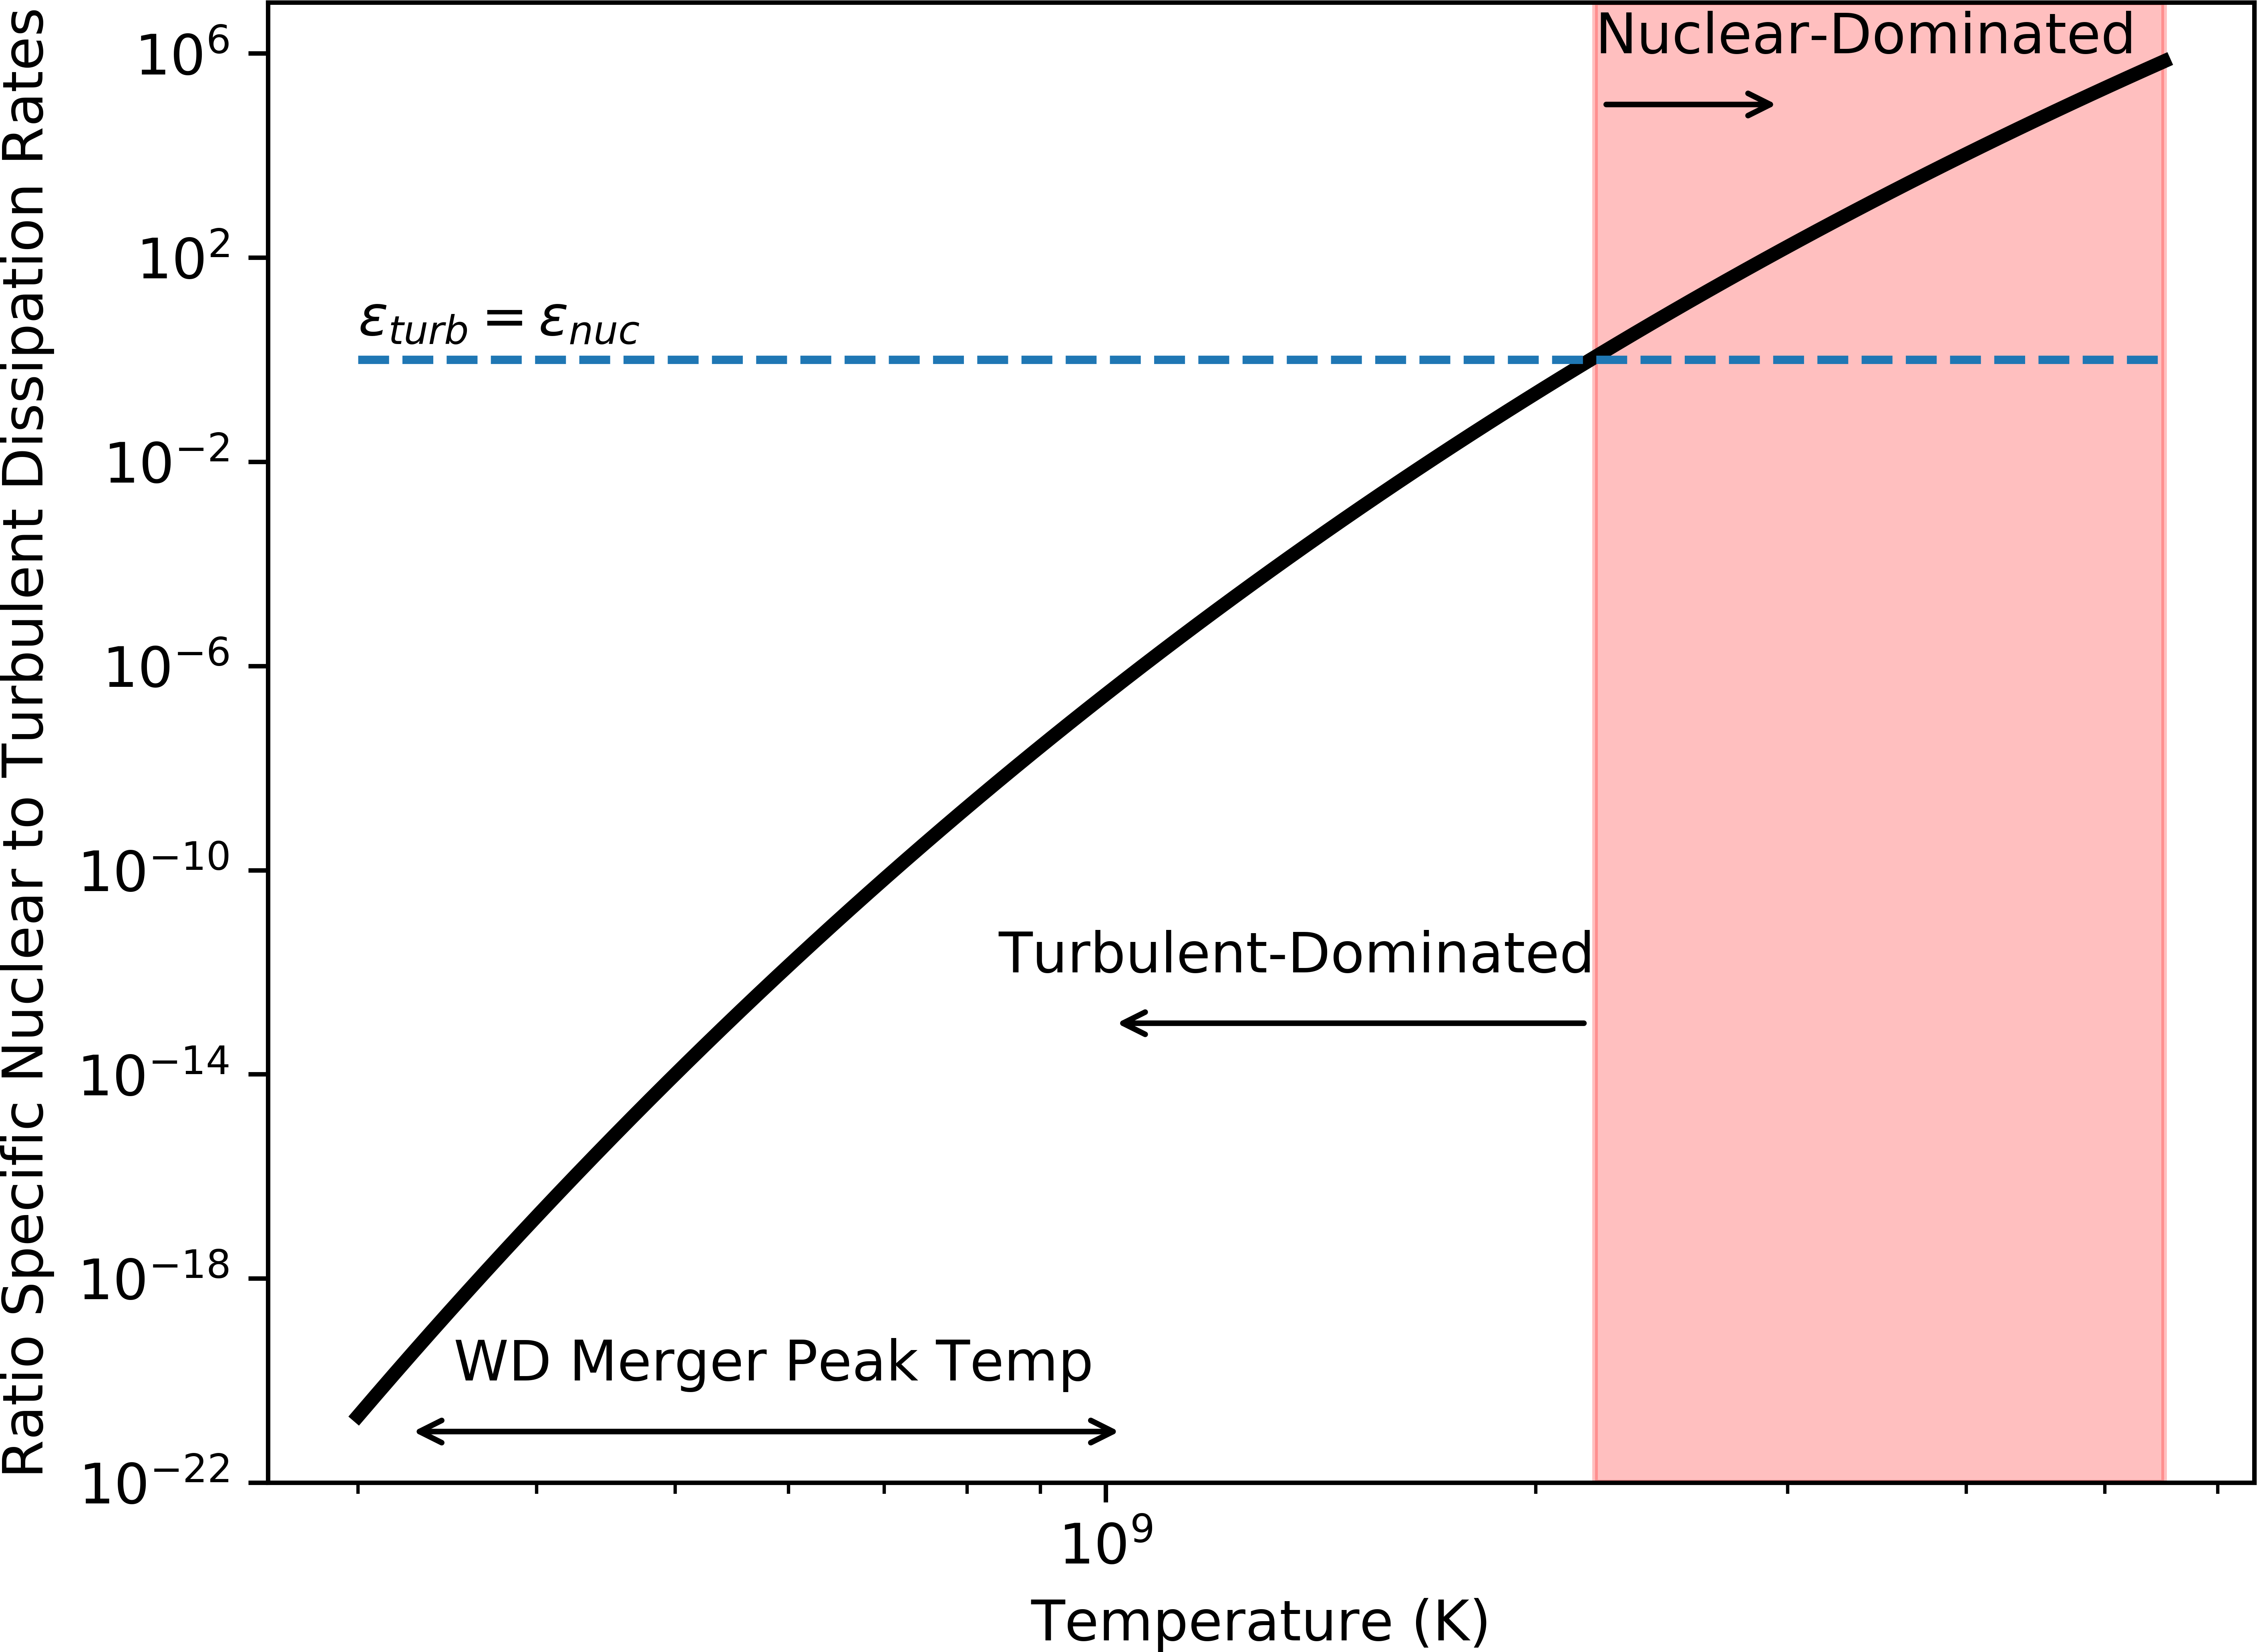
\includegraphics[width=.90\linewidth]{carbon_enuc_ration.png}
            \caption{Analytic Curve for Carbon Detonation}
    \end{center}
  \end{figure}

        \end{columns}

\end{frame}

%------------------------------------------------

\begin{frame}
\frametitle{Carbon Detonation}

        \begin{figure}
    \begin{center}
           \inlineMovie[loop&autostart]{doodoo.mp4}{doodoo.png}{height=0.7\textheight}
    \end{center}
  \end{figure}


\end{frame}

%------------------------------------------------

%------------------------------------------------

\begin{frame}
\frametitle{Carbon Detonation}

        \begin{figure}
    \begin{center}
      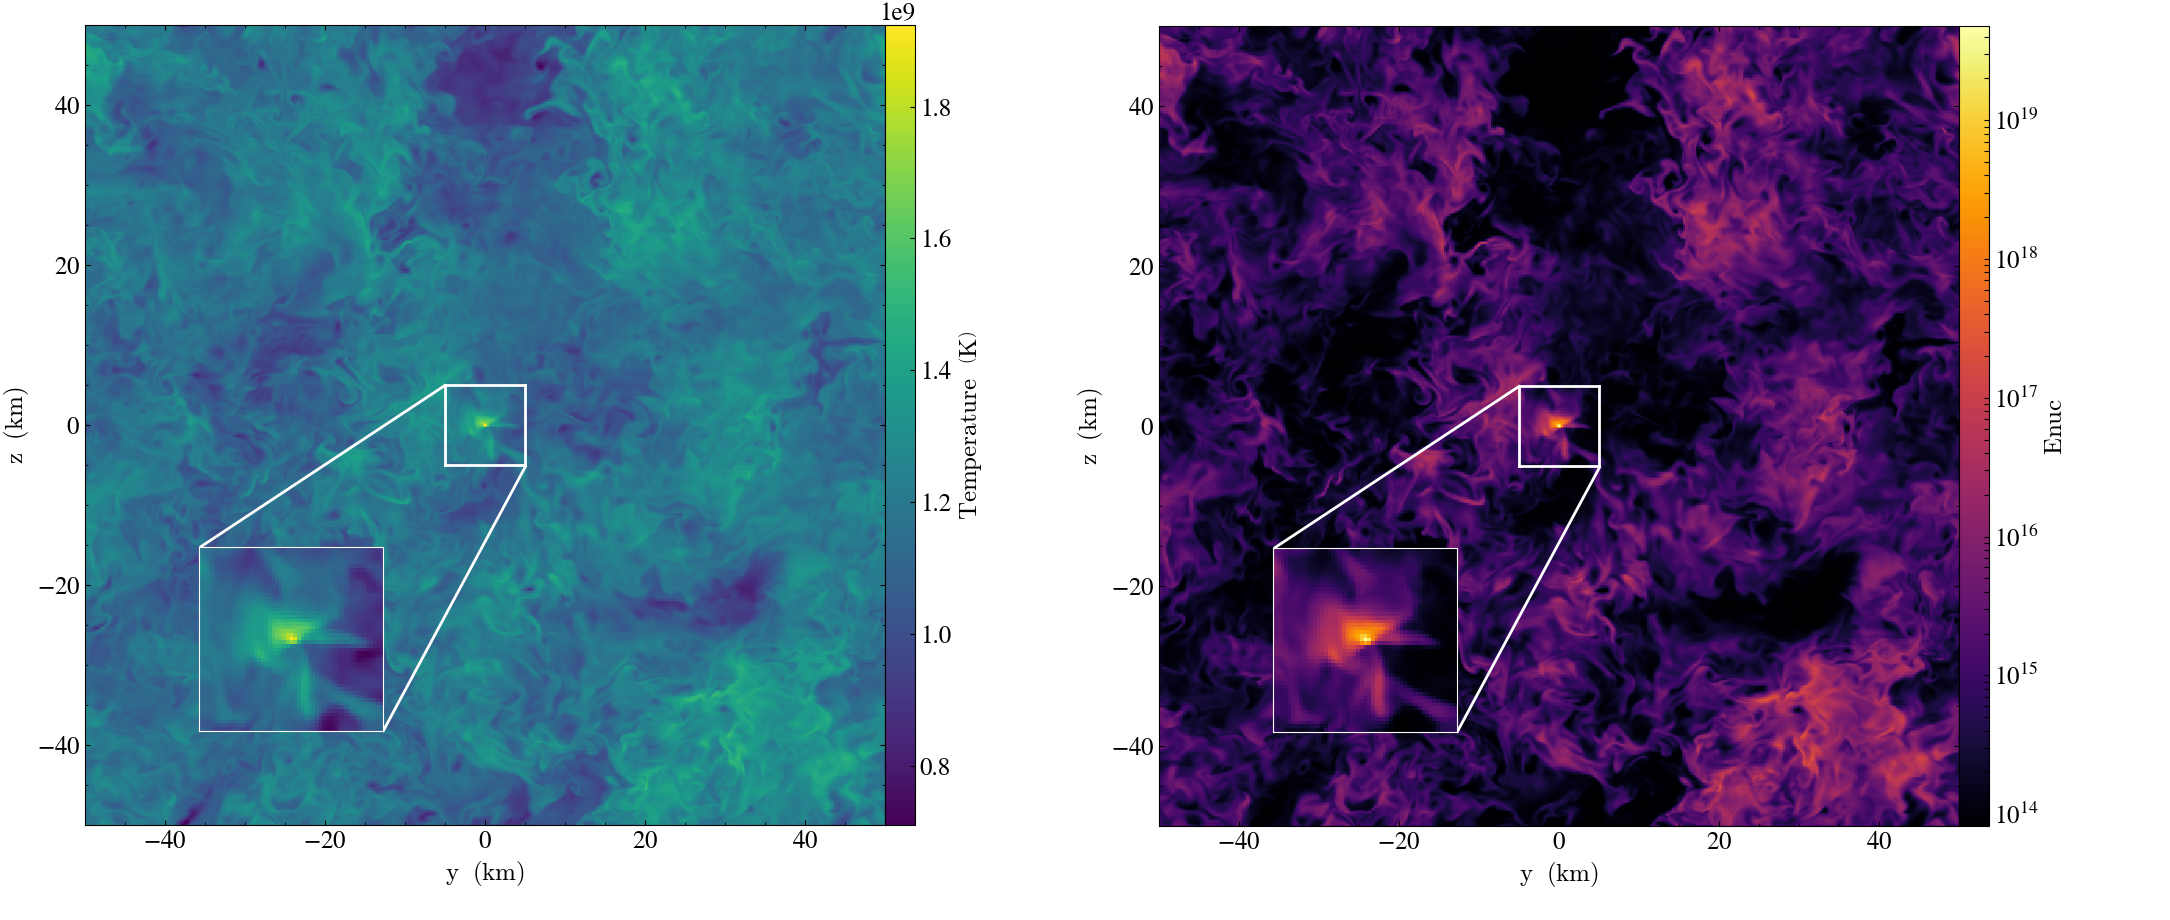
\includegraphics[width=.90\linewidth]{slice.png}
    \end{center}
		\begin{center}
			Slice plots at the moment of detonation.
		\end{center}
  \end{figure}


\end{frame}

%------------------------------------------------


\begin{frame}

        \frametitle{Helium Detonation}
        \begin{center}
        \inlineMovie[loop&autostart]{vishal2.mov}{vishal2.png}{height=0.7\textheight}
		\end{center}
		\begin{center}
			Vishal Tiwari (2019)
		\end{center}
\end{frame}

%------------------------------------------------

\begin{frame}
	\frametitle{Helium Detonation}

        \begin{center}
        \inlineMovie[loop&autostart]{d1.mp4}{d1.png}{height=0.35\textheight}
        \end{center}
	\begin{center}
		NASA, ESA and P. Ruiz-Lapuente, cut and colored by S. Geier
	\end{center}
\end{frame}

%------------------------------------------------

\begin{frame}
\frametitle{Nuclear Physics}

        \begin{figure}
    \begin{center}
      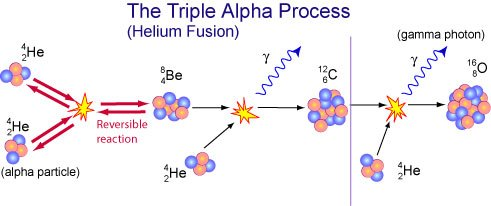
\includegraphics[width=.90\linewidth]{triplealphaflash.jpg}
    \end{center}
  \end{figure}

\end{frame}

%------------------------------------------------

\begin{frame}
\frametitle{Method}

\begin{columns}[c]
        \column{0.5\textwidth}
        \begin{itemize}
                \item 3D Models
                \item 100km periodic box
		\item Uniform Grid
		\item Driving force for turbulence on a large scale
		\item Helmholtz Equation of State
		\item 19-isotope network
        \end{itemize}


\column{0.5\textwidth}
        \vspace{25pt}
        \begin{figure}
    \begin{center}
      \includegraphics[width=.90\linewidth]{grid_transp.png}
    \end{center}
  \end{figure}

        \end{columns}

\end{frame}


%------------------------------------------------

\begin{frame}
\frametitle{Method}

\begin{columns}[c]
        \column{0.5\textwidth}
        \begin{itemize}
                \item Resolution set to $128^3, 256^3, 512^3, 1024^3$
                \item Mass density set to $10^5, 10^6 (\frac{g}{cm^3}$)
		\item Helium fraction set to $1.0, 0.25, 0.1$
                \item Used FLASH4 code on Stampede2
        \end{itemize}


\column{0.5\textwidth}
        \vspace{25pt}
        \begin{figure}
    \begin{center}
      \includegraphics[width=.90\linewidth]{grid_transp.png}
    \end{center}
  \end{figure}

        \end{columns}

\end{frame}

%------------------------------------------------


\begin{frame}
	
	\frametitle{Results}
	\begin{center}
	\inlineMovie[loop&autostart]{out.mp4}{out.png}{height=0.7\textheight}
	\end{center}
	\begin{center} 
		Detonation of $128^{3}$ run with $\rho = 10^6 \frac{g}{cm^3}$ and He fraction = 0.25.
	\end{center}
\end{frame}

%------------------------------------------------
\begin{frame}
	\frametitle{Results}
	\begin{itemize}
		\item Triple Alpha is more sensitive to density than carbon burning
		\item Helium detonation occurs sooner than carbon
		\item Alpha capture onto carbon and oxygen dominates at later times
	\end{itemize}
\end{frame}

%-----------------------------------------------

\begin{frame}
	\frametitle{Future Work}
	\begin{itemize}
		\item Incorporate higher isotope network
		\item Keep exploring parameter space
		\item Nitrogen, Neon
		\item Expand these sub-grid models into global situations
	\end{itemize}
\end{frame}




\end{document}
